\chapter{Results}
As all the necessary requirements for the PEEPS framework presented in 3.1.2 were fulfilled, testing on both the application and server systems could commence. The experimental setup and findings for this project are detailed in this section.


\section{Final Product Presentation}
The final product was tested on a OnePlus 7 Pro smartphone with its GPS and network location services enabled. The device contains a Snapdragon 855 processor, a 1440p display and 6GB of RAM.

\begin{figure}
    \centering
    \begin{minipage}{.5\textwidth}
      \centering
      \frame{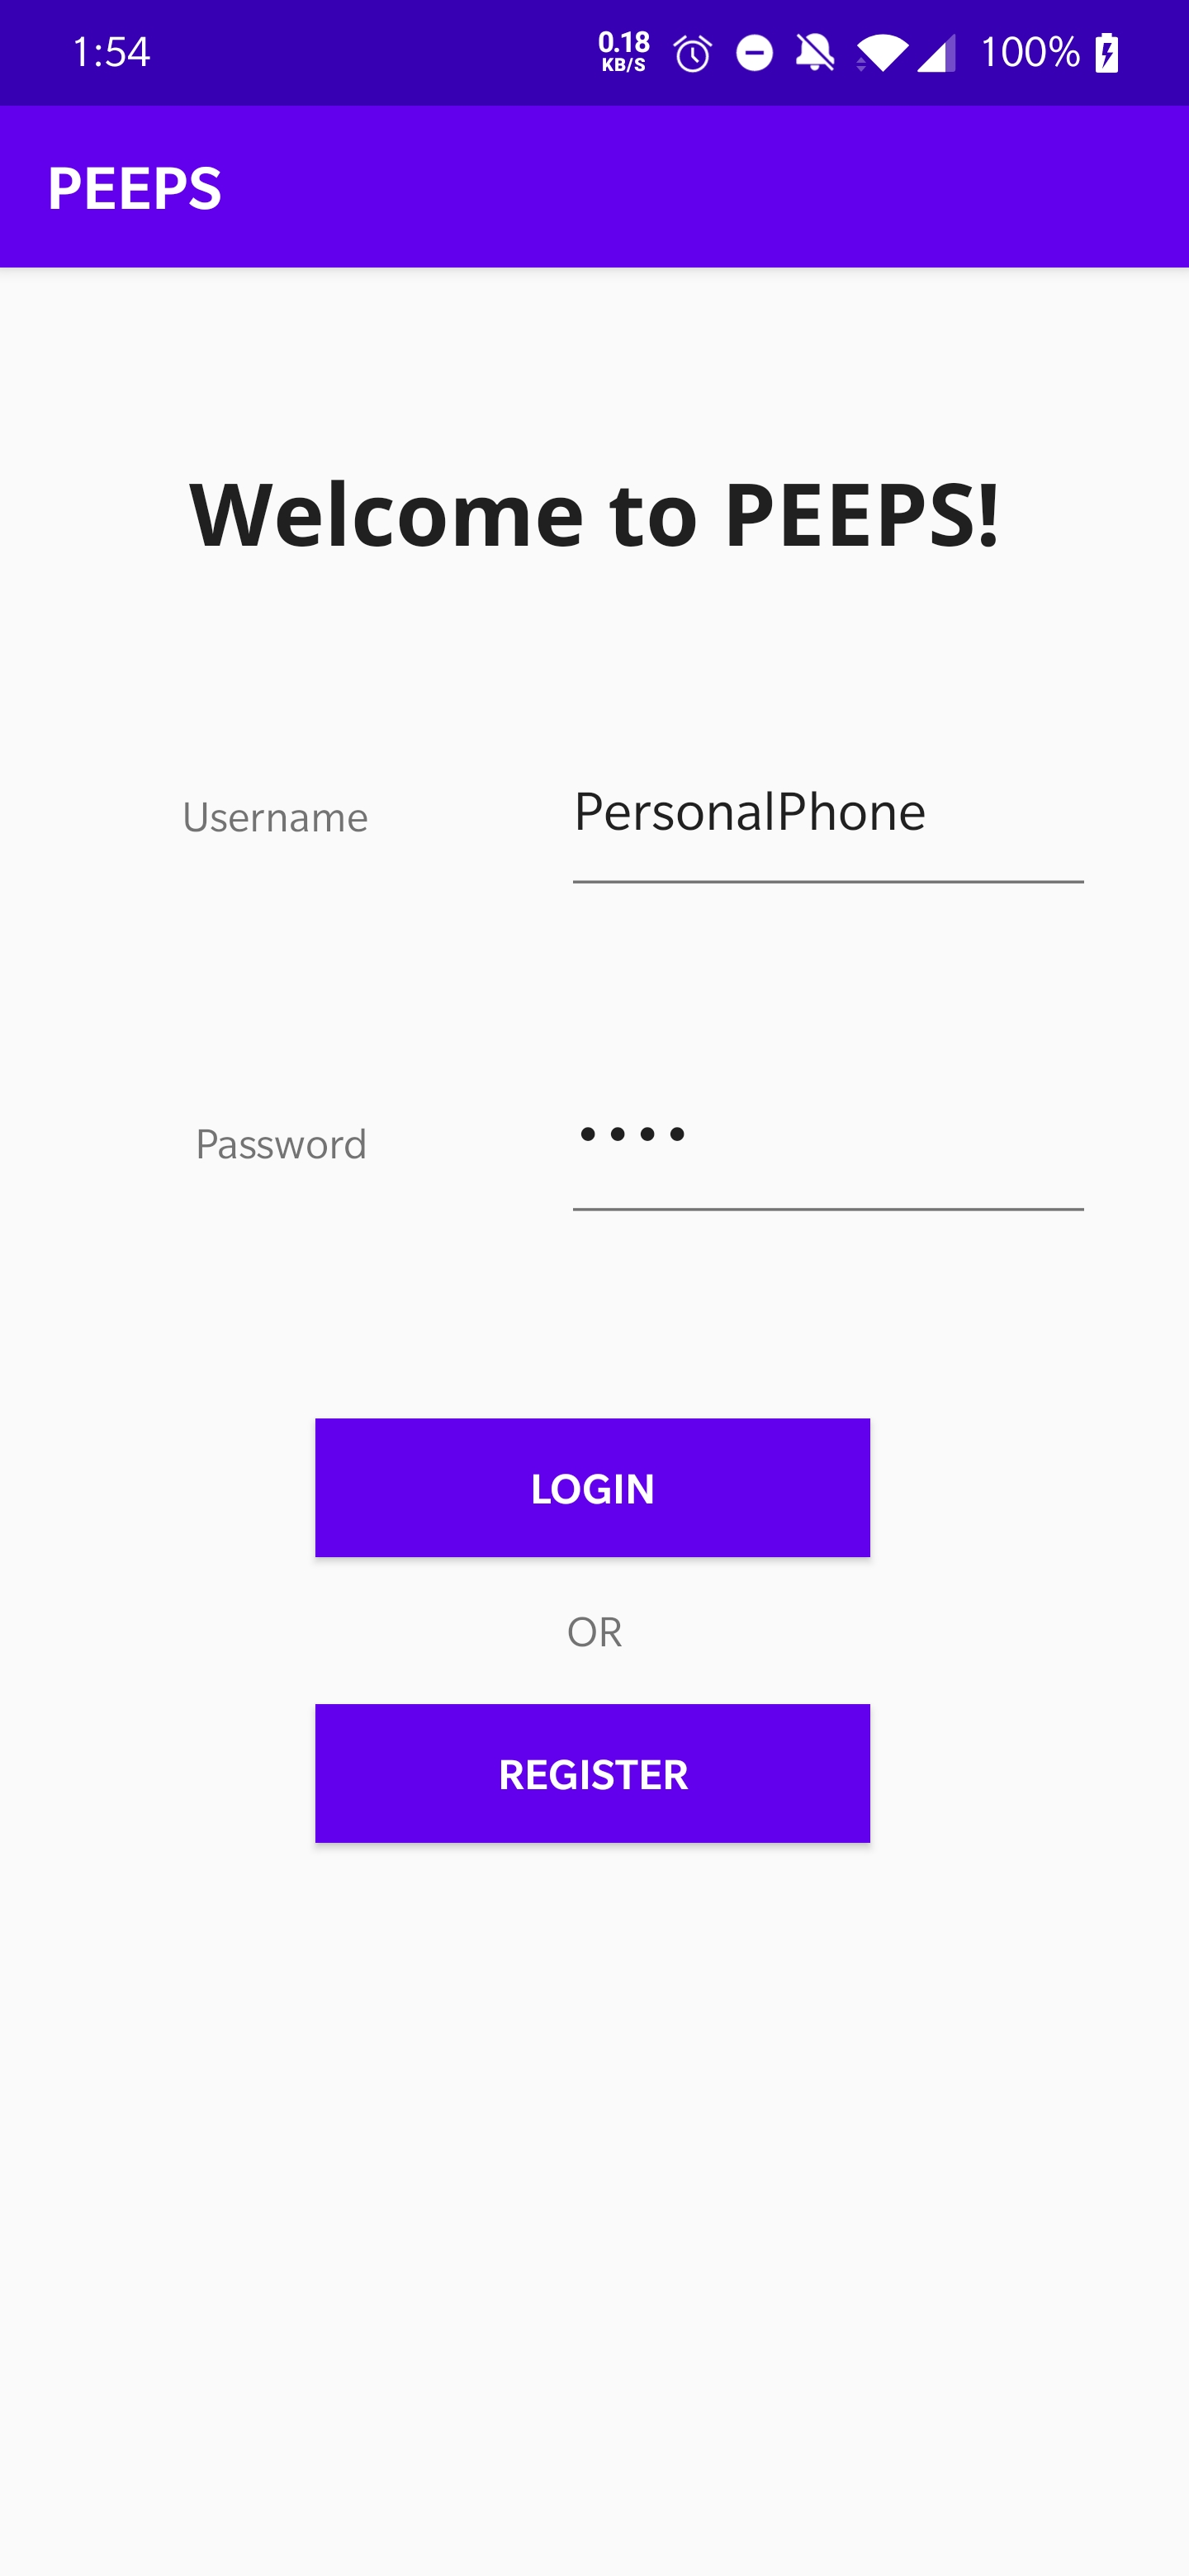
\includegraphics[width=.6\linewidth]{figures/ResultLogin.jpg}}
      \caption{Final product login view.}
      \label{fig:results_login}
    \end{minipage}%
    \begin{minipage}{.5\textwidth}
      \centering
      \frame{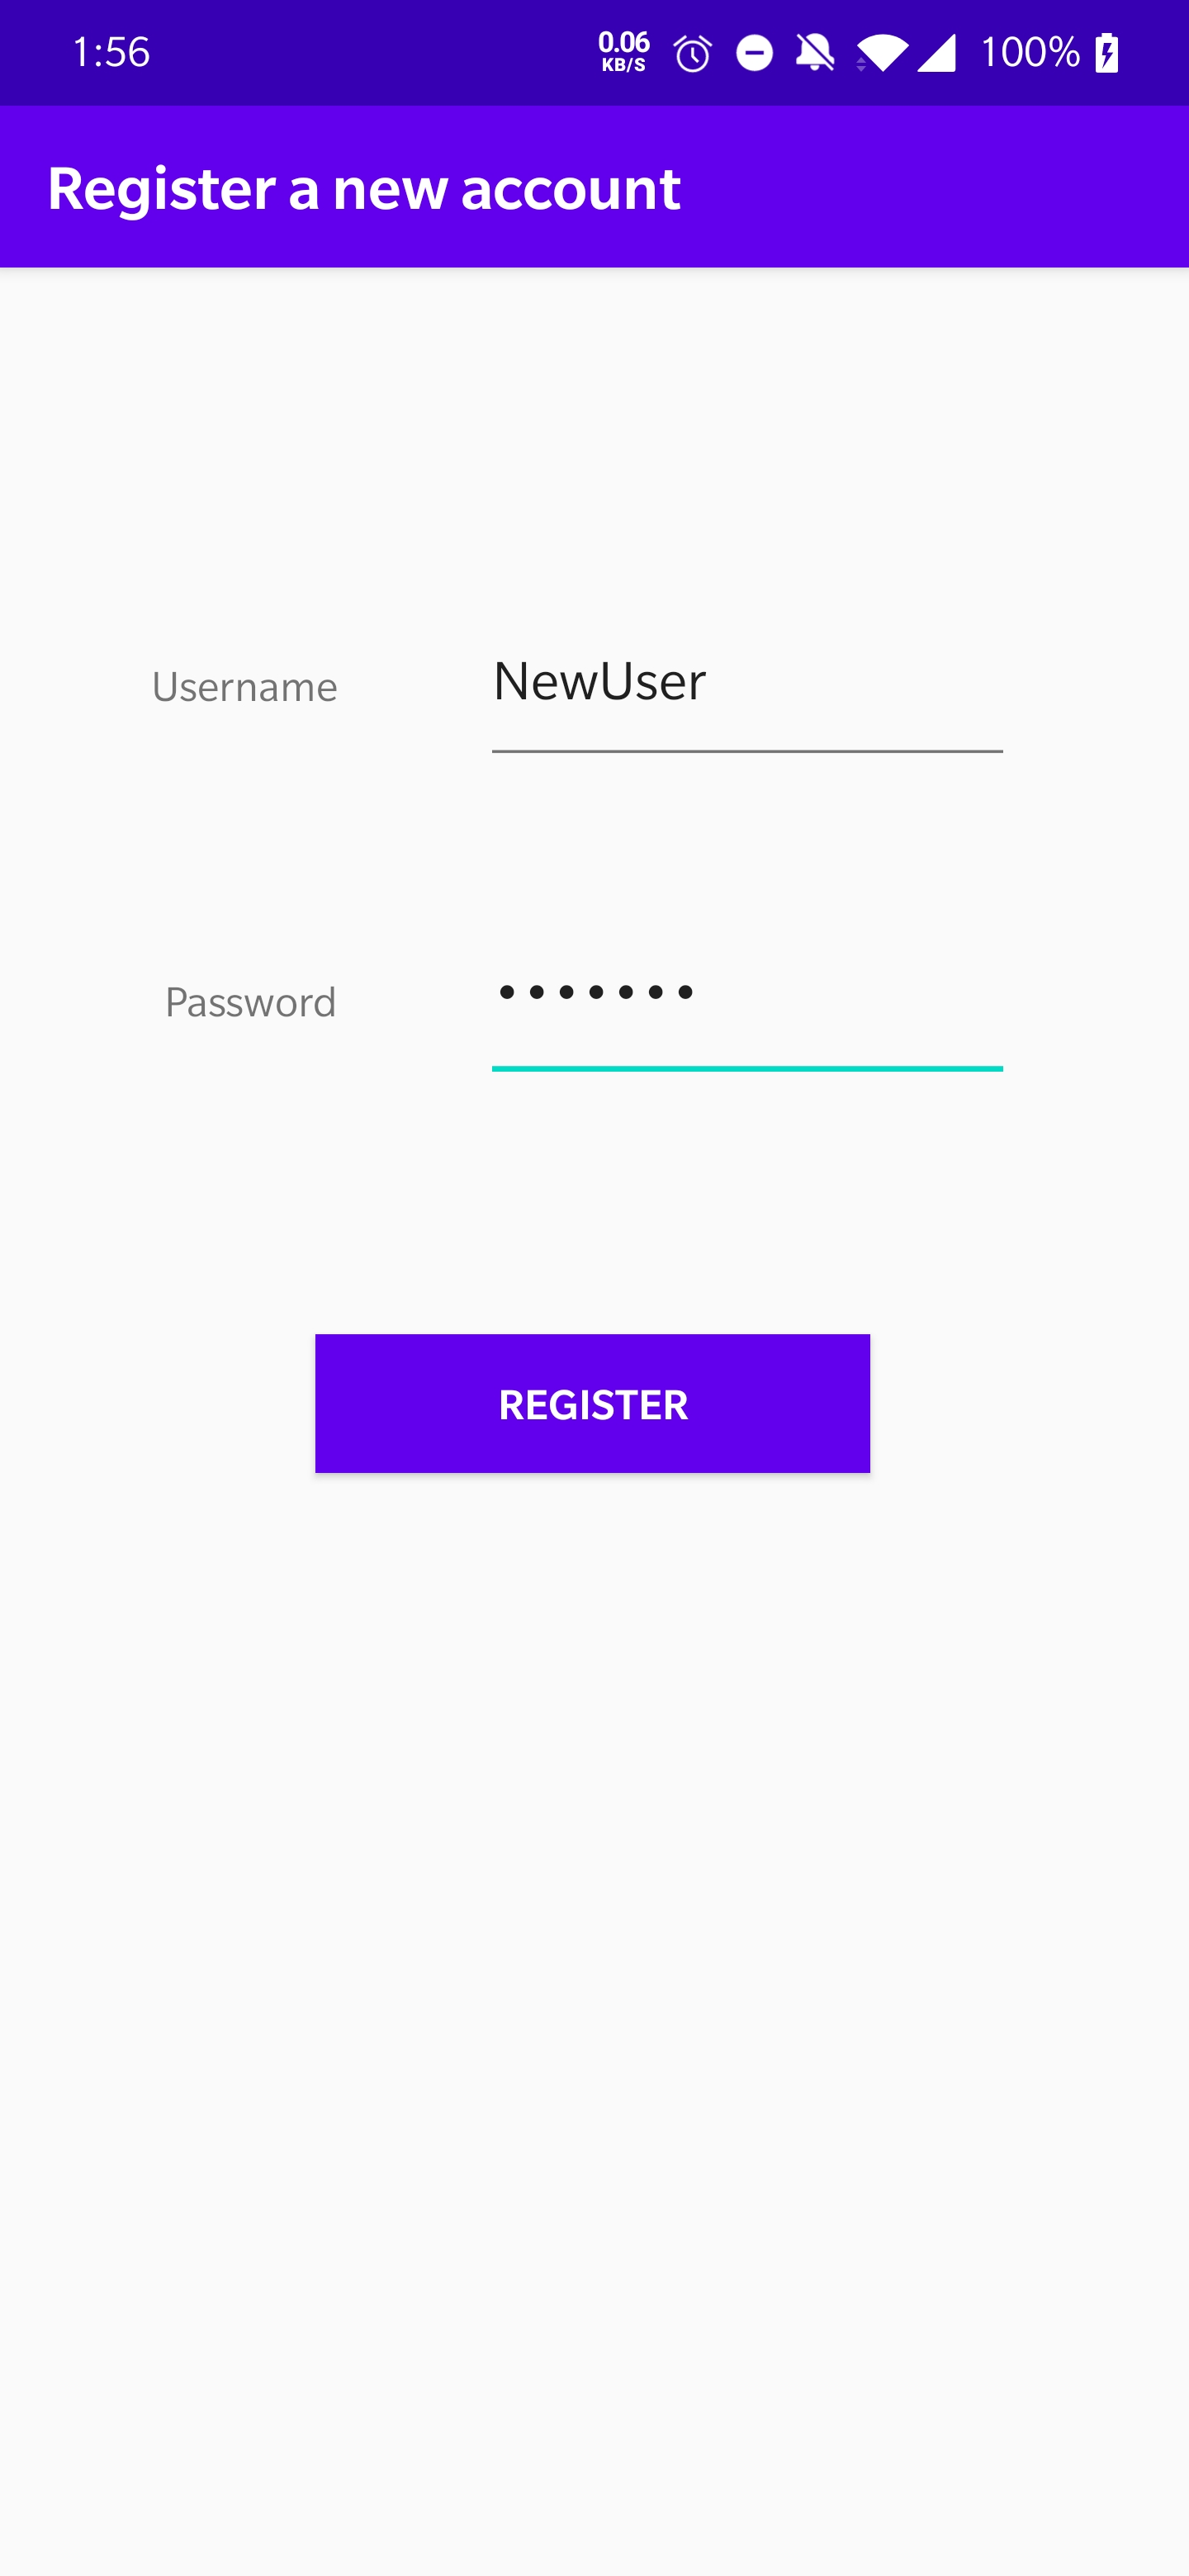
\includegraphics[width=.6\linewidth]{figures/ResultRegister.jpg}}
      \caption{Final product register-user view.}
      \label{fig:result_register}
    \end{minipage}
\end{figure}

The login and register GUIs are built with simplicity and usability as their core design principles. The input fields are centred and take up most of the screen's interactive space, while the actions that the user can take are displayed as highly contrasted buttons. These views also highlight the theme that was decided for this app which is a clean light grey background with purple interactable elements. 

\begin{figure}
    \centering
    \begin{minipage}{.5\textwidth}
      \centering
      \frame{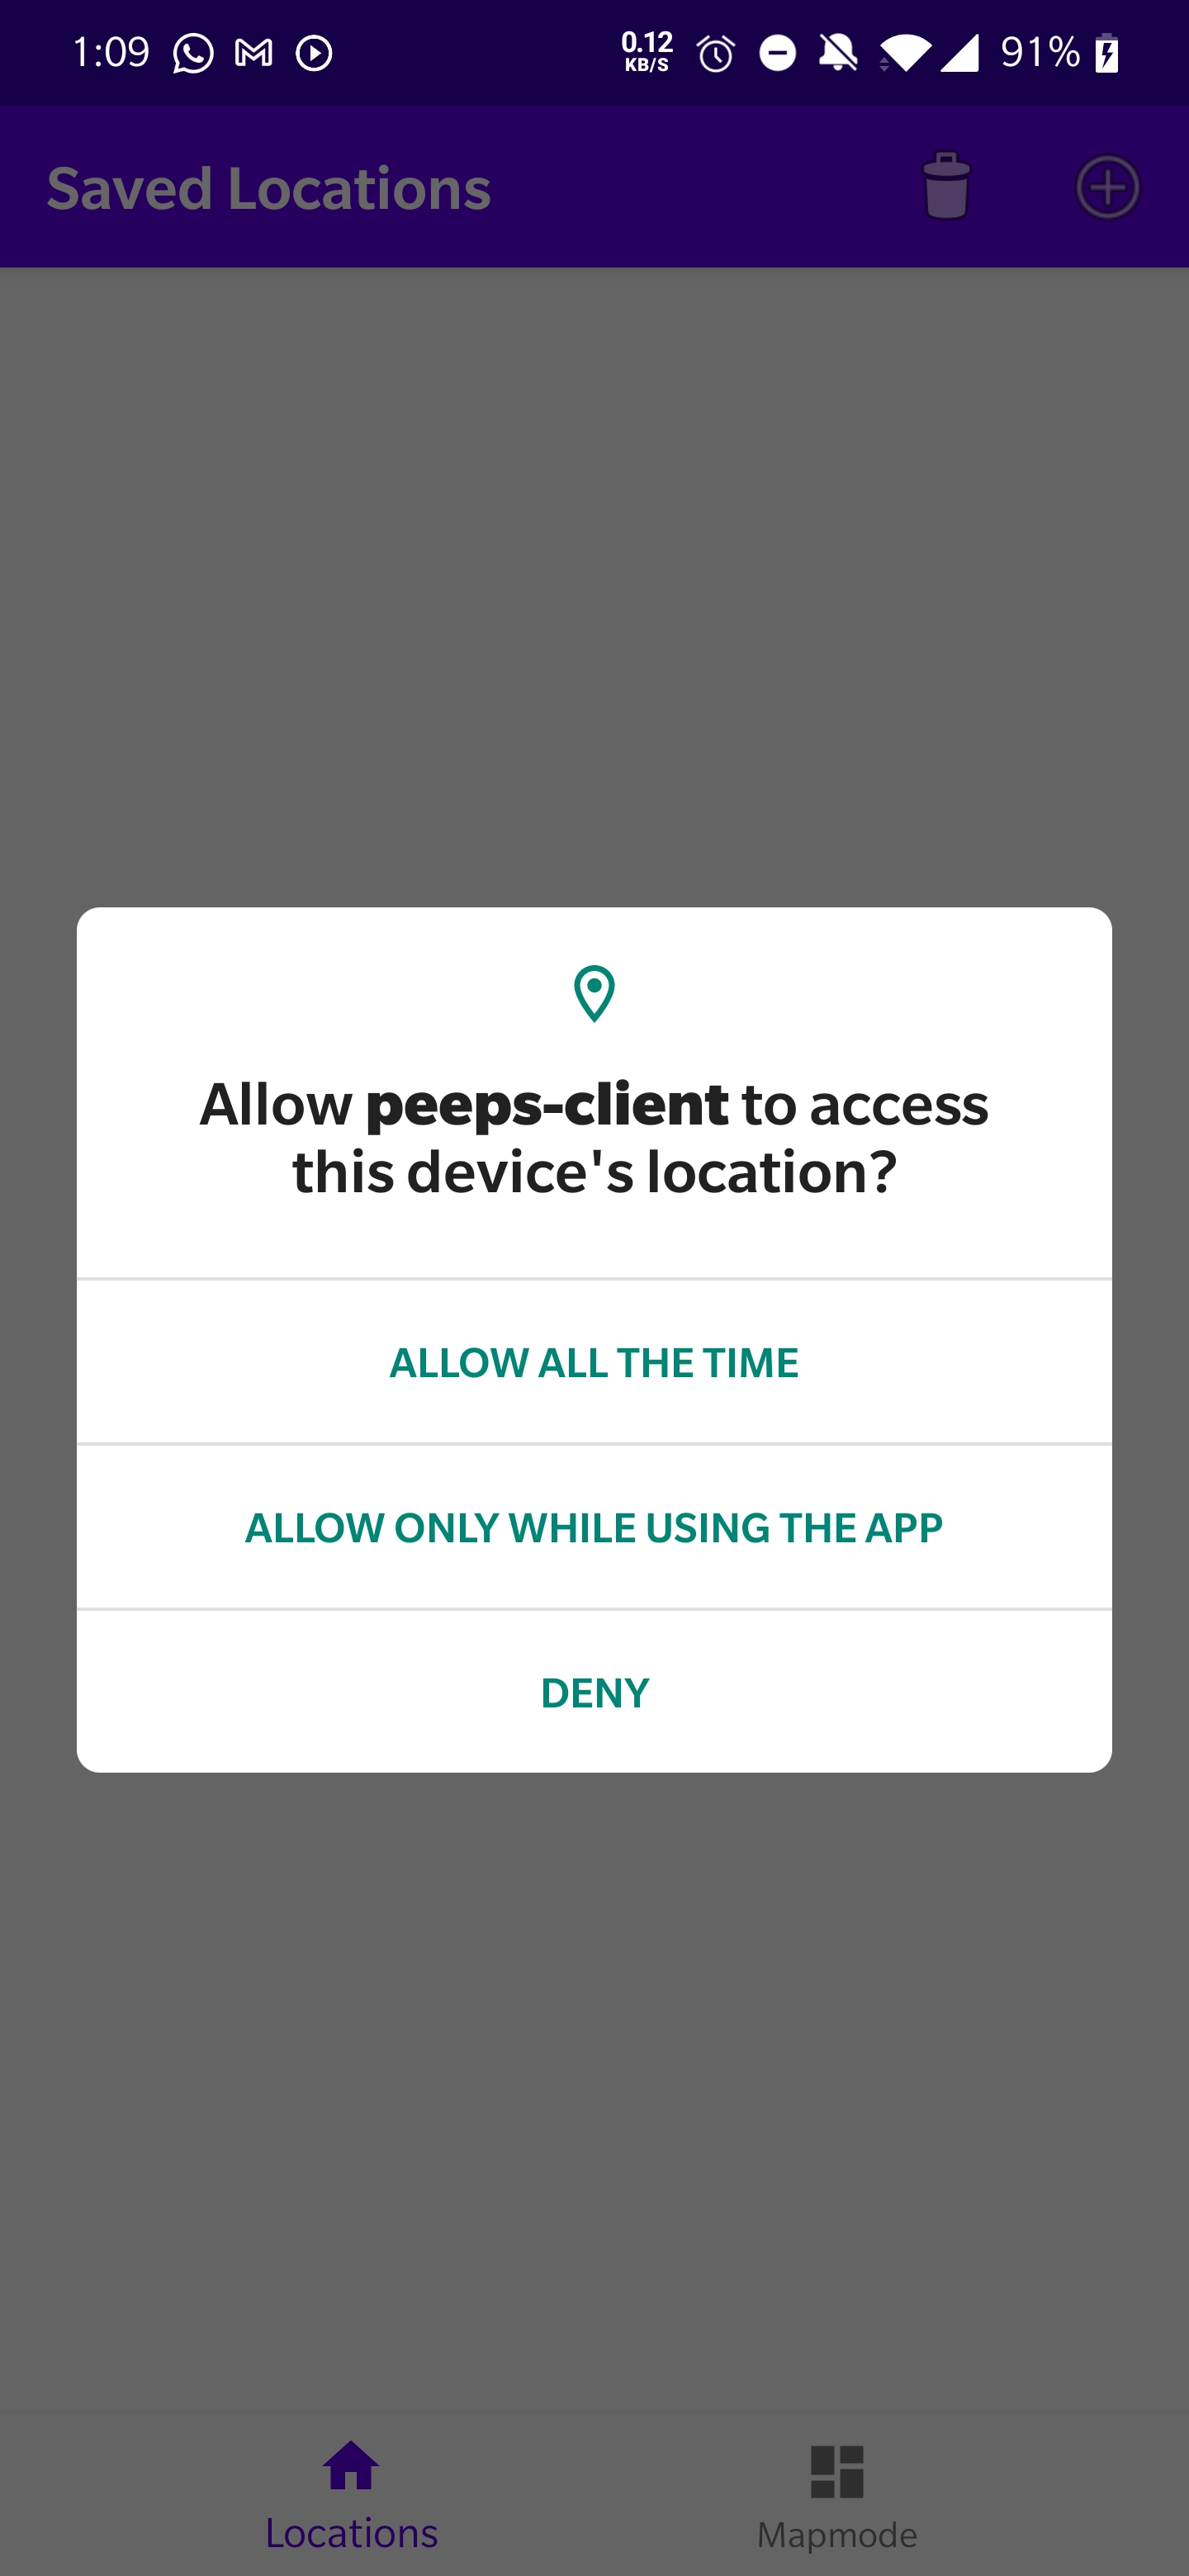
\includegraphics[width=.6\linewidth]{figures/ResultPermission.jpg}}
      \caption{Location permission alert shown when user first logs in.}
      \label{fig:result_permission}
    \end{minipage}%
    \begin{minipage}{.5\textwidth}
        When the user first logs into the app after creating an account, they will be asked to allow the app to access their location. Without this feature, the user will not be able to contribute their location to the crowd sourcing database. The app will however still function without this feature enabled.
    \end{minipage}
\end{figure}

\begin{figure}
    \centering
    \begin{minipage}{.5\textwidth}
      \centering
      \frame{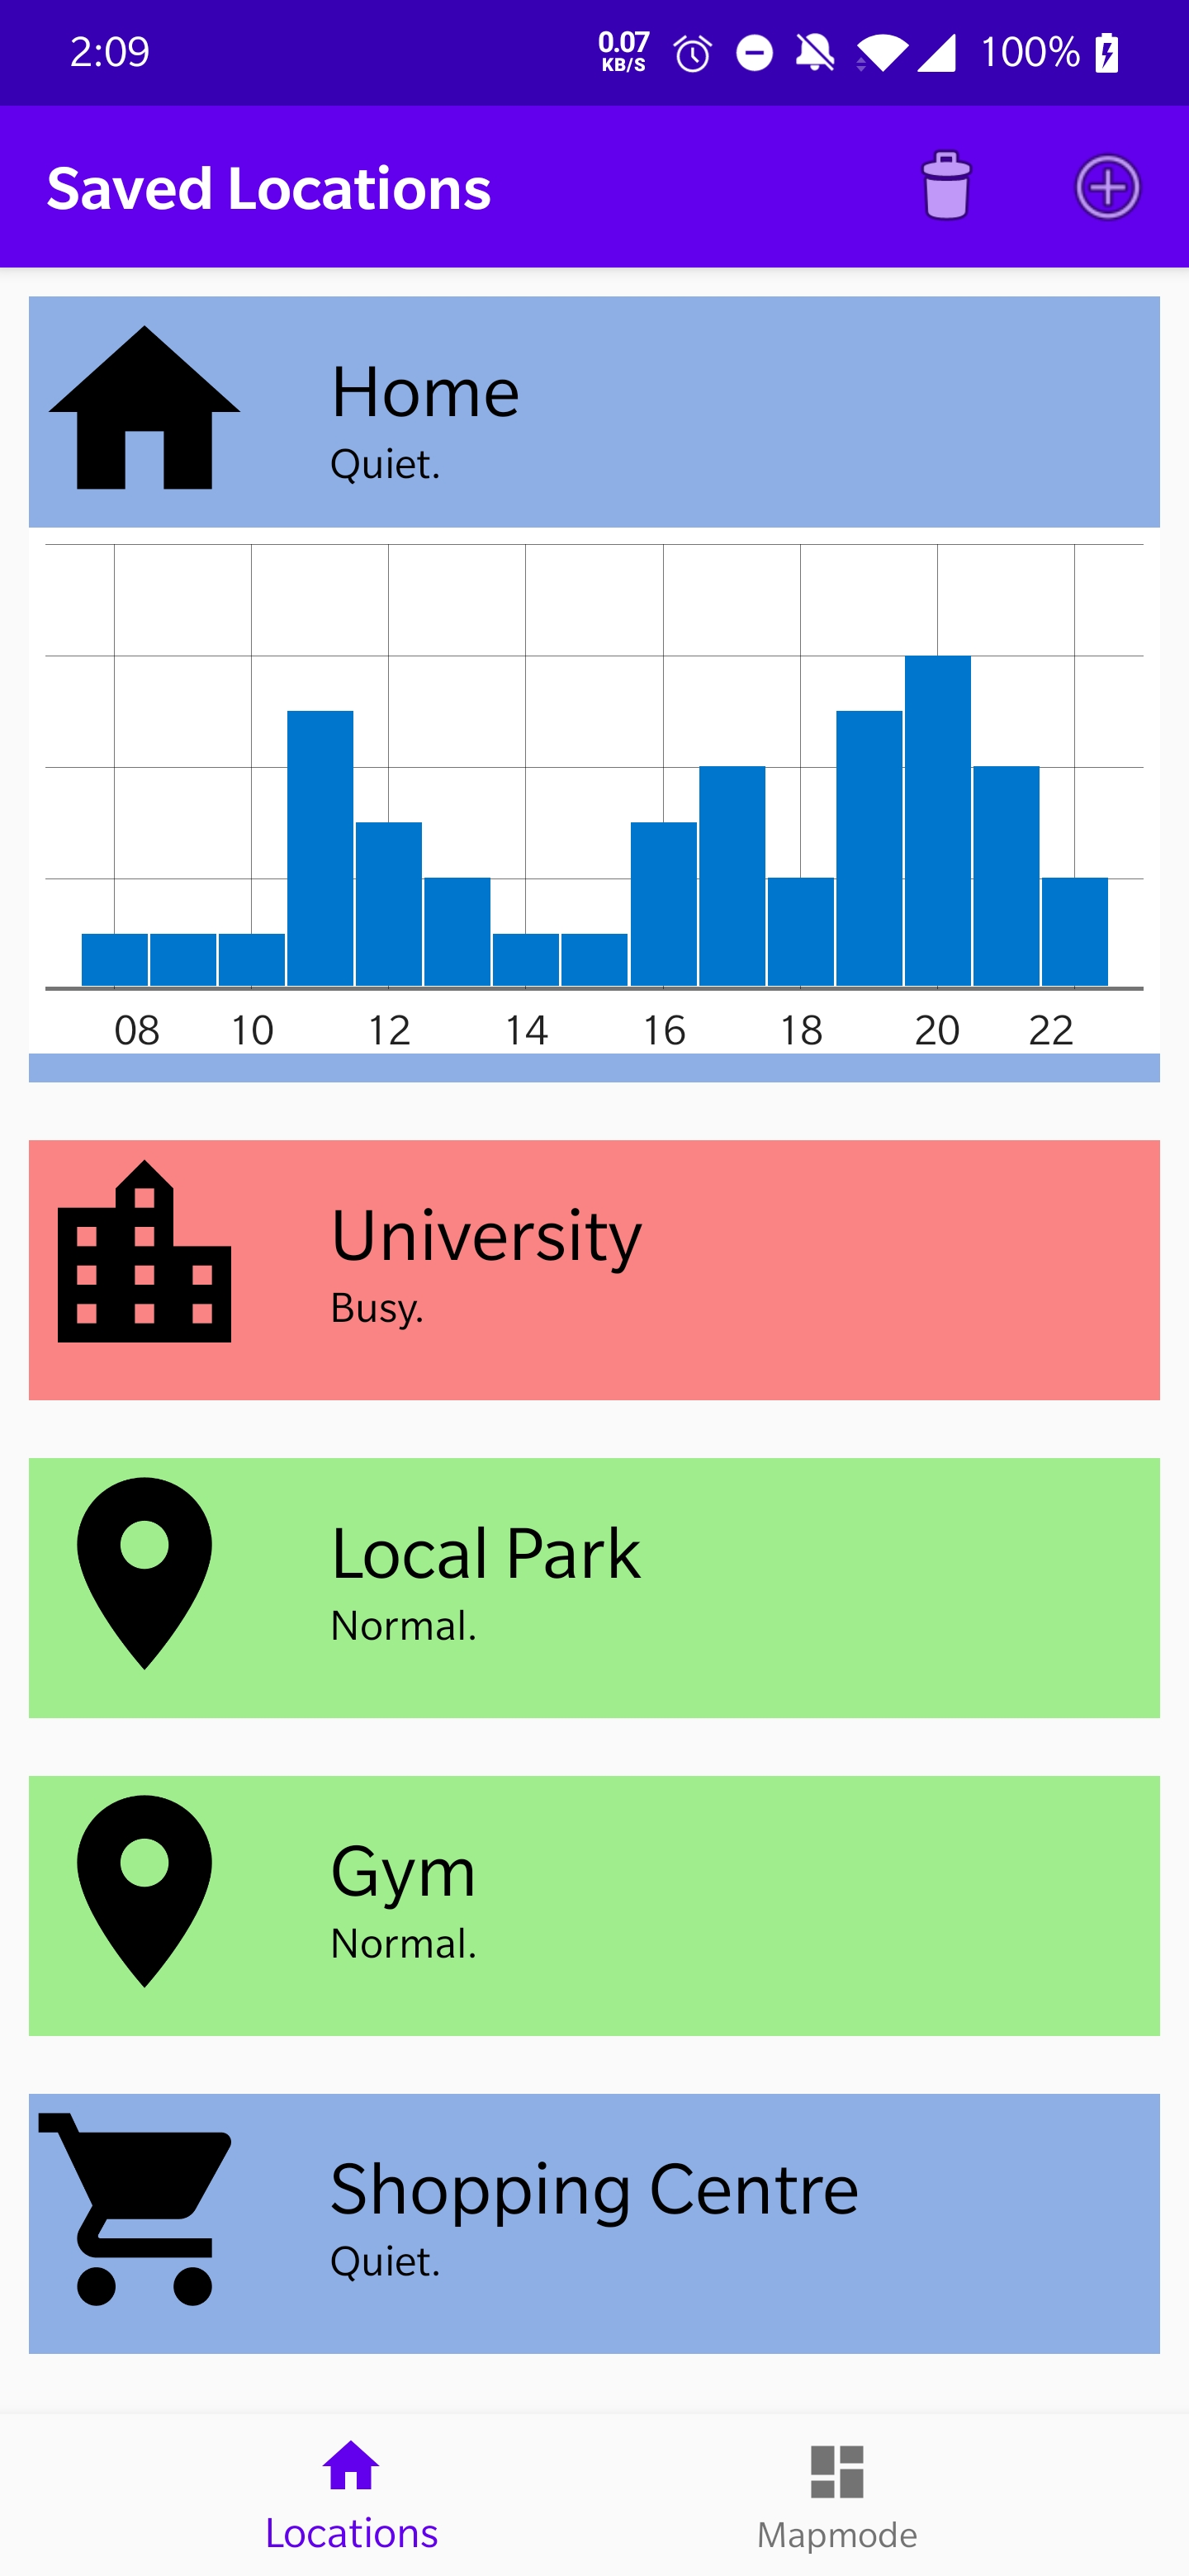
\includegraphics[width=.6\linewidth]{figures/ResultExtended.jpg}}
      \caption{Saved-location view with\\first location extended.}
      \label{fig:result_extended}
    \end{minipage}%
    \begin{minipage}{.5\textwidth}
      \centering
      \frame{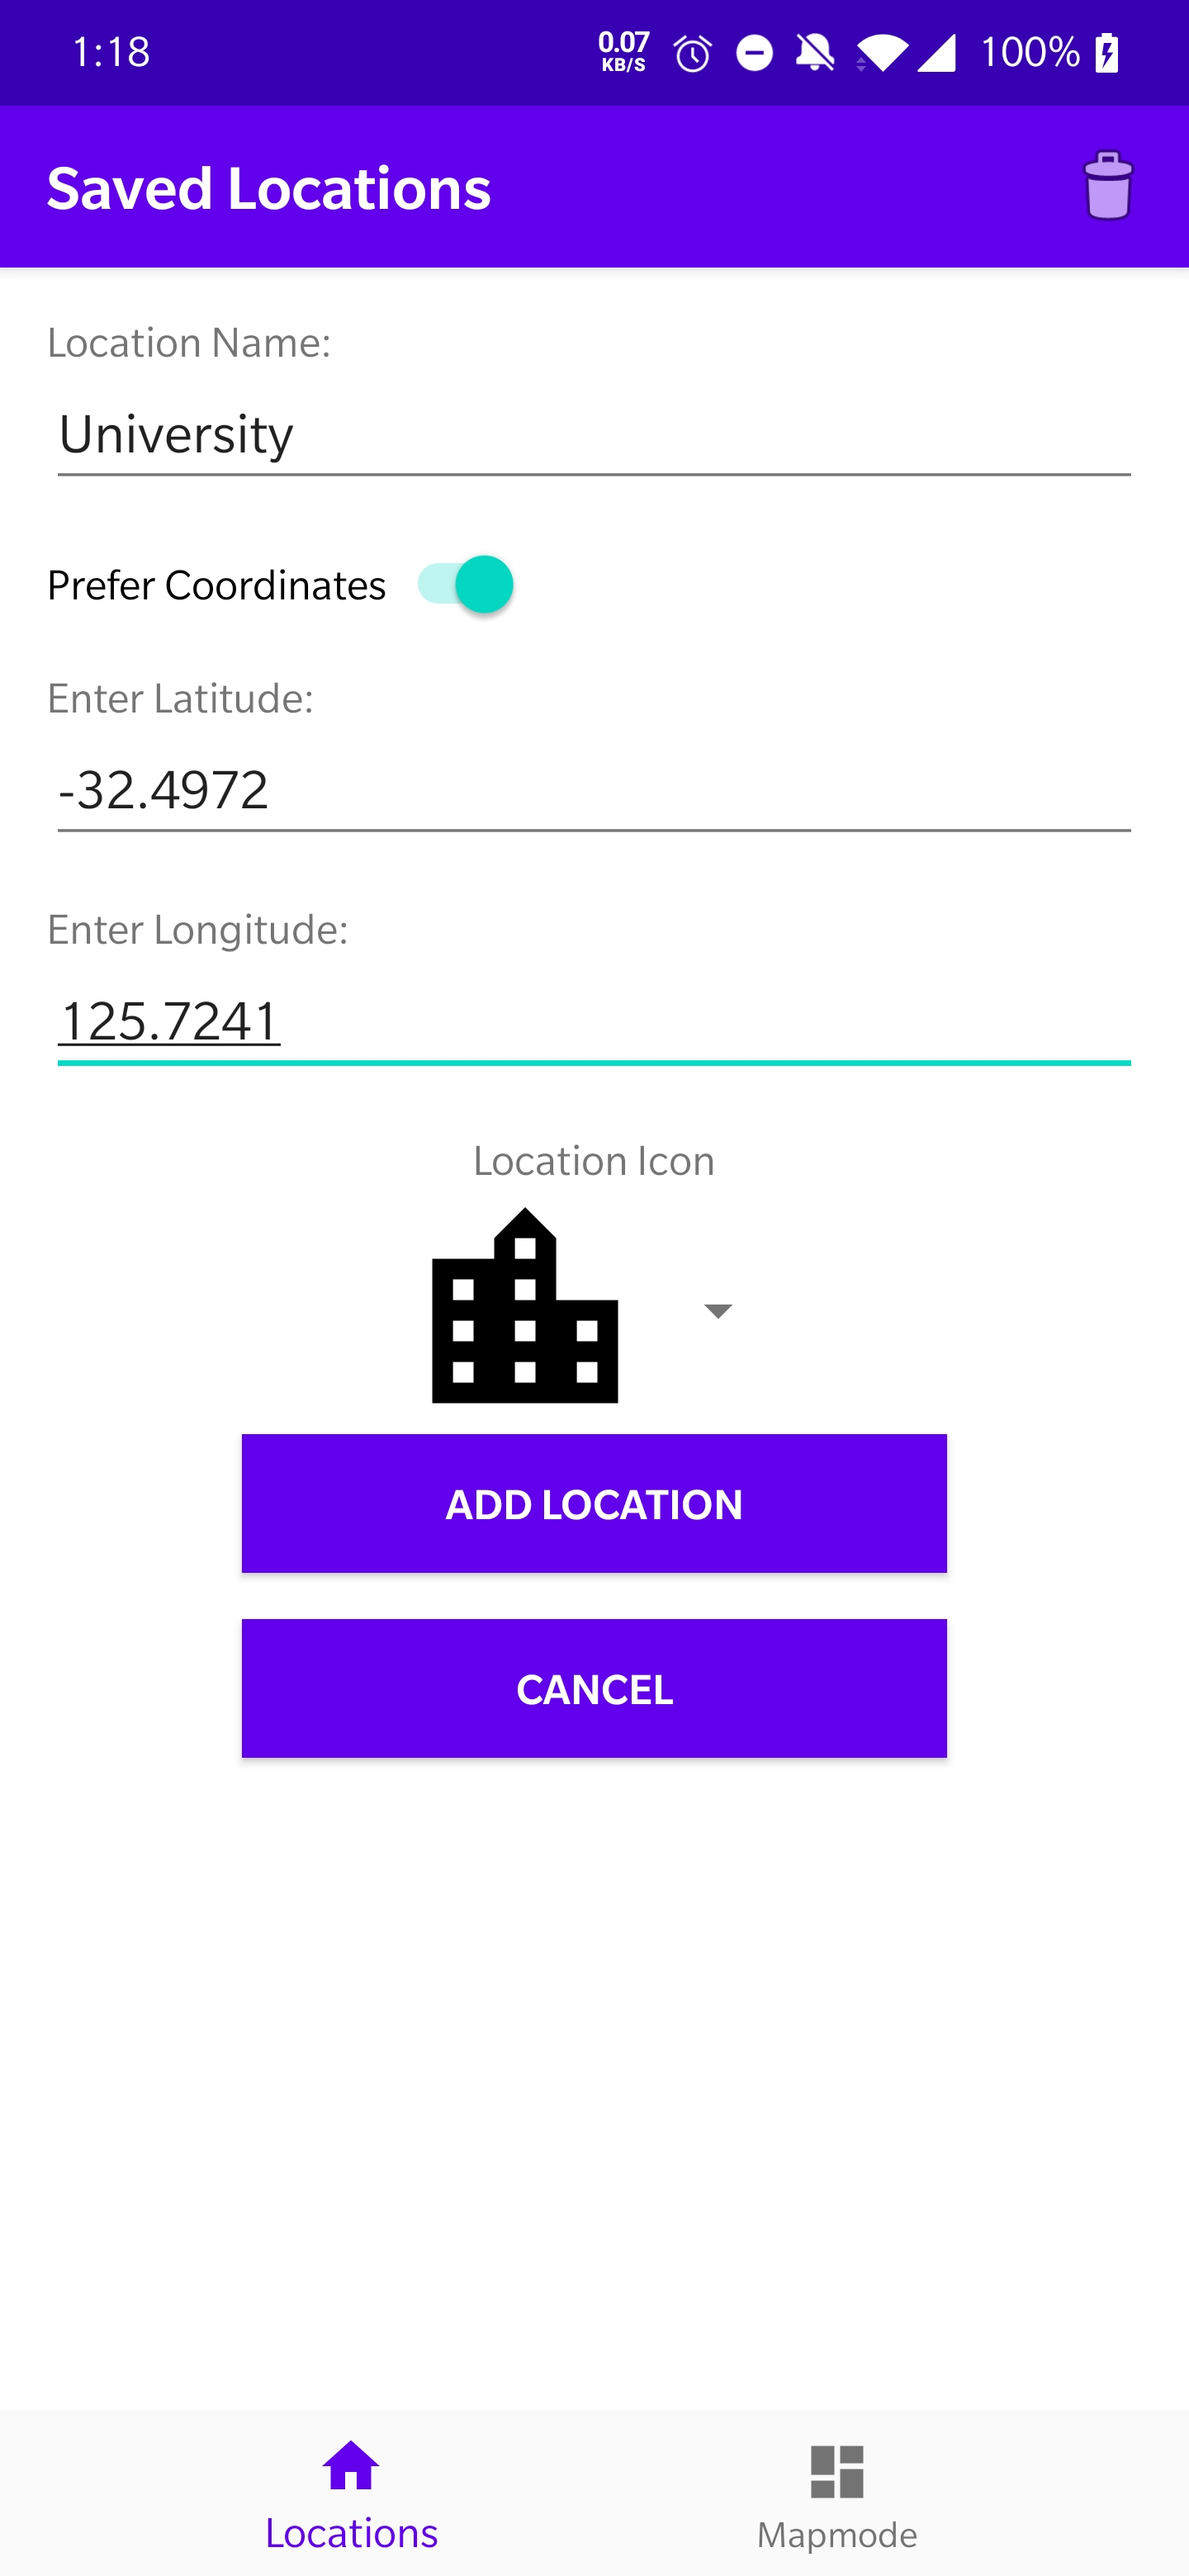
\includegraphics[width=.6\linewidth]{figures/ResultAdd.jpg}}
      \caption{Saved-location dialog fragment.}
      \label{fig:result_add}
    \end{minipage}
\end{figure}

The views in Figure \ref{fig:result_extended} and Figure \ref{fig:result_add} show the main functionality of the application. Figure \ref{fig:result_extended} is the main page of the Population-Denisty Activity, displaying the user's saved locations and their current population status. For the purpose of testing, these locations' population data were artificially inserted into the database to provide insight into how the app would look under actual usage conditions. Figure \ref{fig:result_add} displays the Dialog Fragment which overlays the view of Figure \ref{fig:result_extended}. Here the user inputs the name, icon, and coordinates of a new location.

The GUI from the mapmode fragment is shown in the results page in Figure \ref{fig:result_mapmode}.

\subsection{Application Interaction Feedback Mechanisms}
It is important when designing a user interface that the user is presented with dynamic methods of interaction to help inform them of the results of their actions. The PEEPS application implements this by utilising `toasts'. These are temporary update messages which inform the user of a background process that they would benefit from knowing about. 

\begin{figure}[ht]
    \centering
    \frame{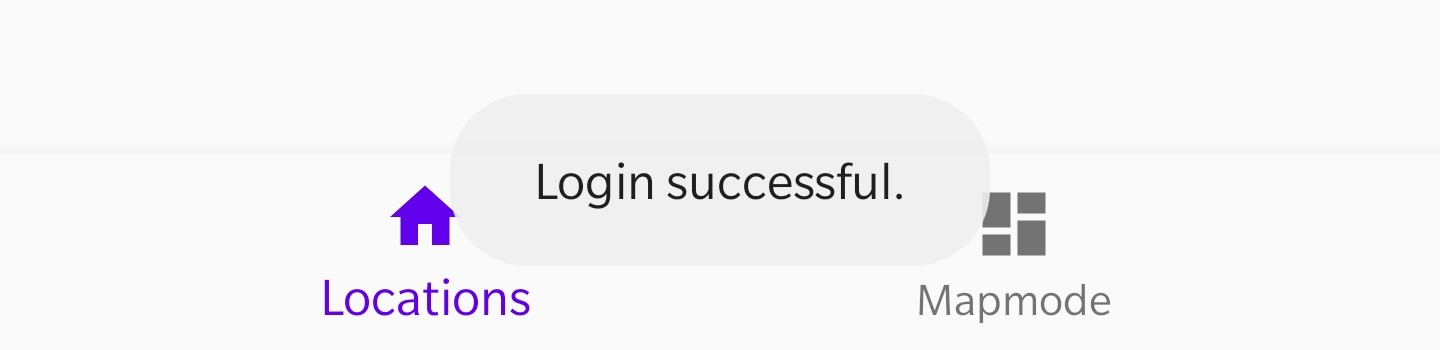
\includegraphics[width=0.7\textwidth]{figures/ResultToast.jpg}}
    \caption{Population-Density Activity's successful login toast.}
    \label{fig:result_toast}
\end{figure}

Another way the application provides feedback to the user is the transition between an item of figure \ref{fig:result_extended} being expanded and closed. When the item is selected, the location card will slowly expand and the graph will become visible. This transition makes the user interaction less sudden and ensures they understand the consequences of selecting an item in the list.

\section{Functional Testing}
TEST-1: \textbf{Location Status Test}

For this first test, a list of user locations was manually added to the database with a constant set of coordinates. The number of locations added to the database was equal to the first number of the time bracket at which their location was hypothetically taken, with a timestamp dating a week earlier than the test day. Because the web interface queries data from three weeks prior to the request, we expect to see a linearly increasing graph displayed on the app when analysing data from the correct coordinates.

While conducting the test, the resulting graph displayed on the app was one with a linearly increasing population. This verifies the app's ability to use the Saved Location View to display accurate information about the status of chosen locations.

TEST-2: \textbf{Best Route Test}

\begin{figure}[!htbp]
    \centering
    \frame{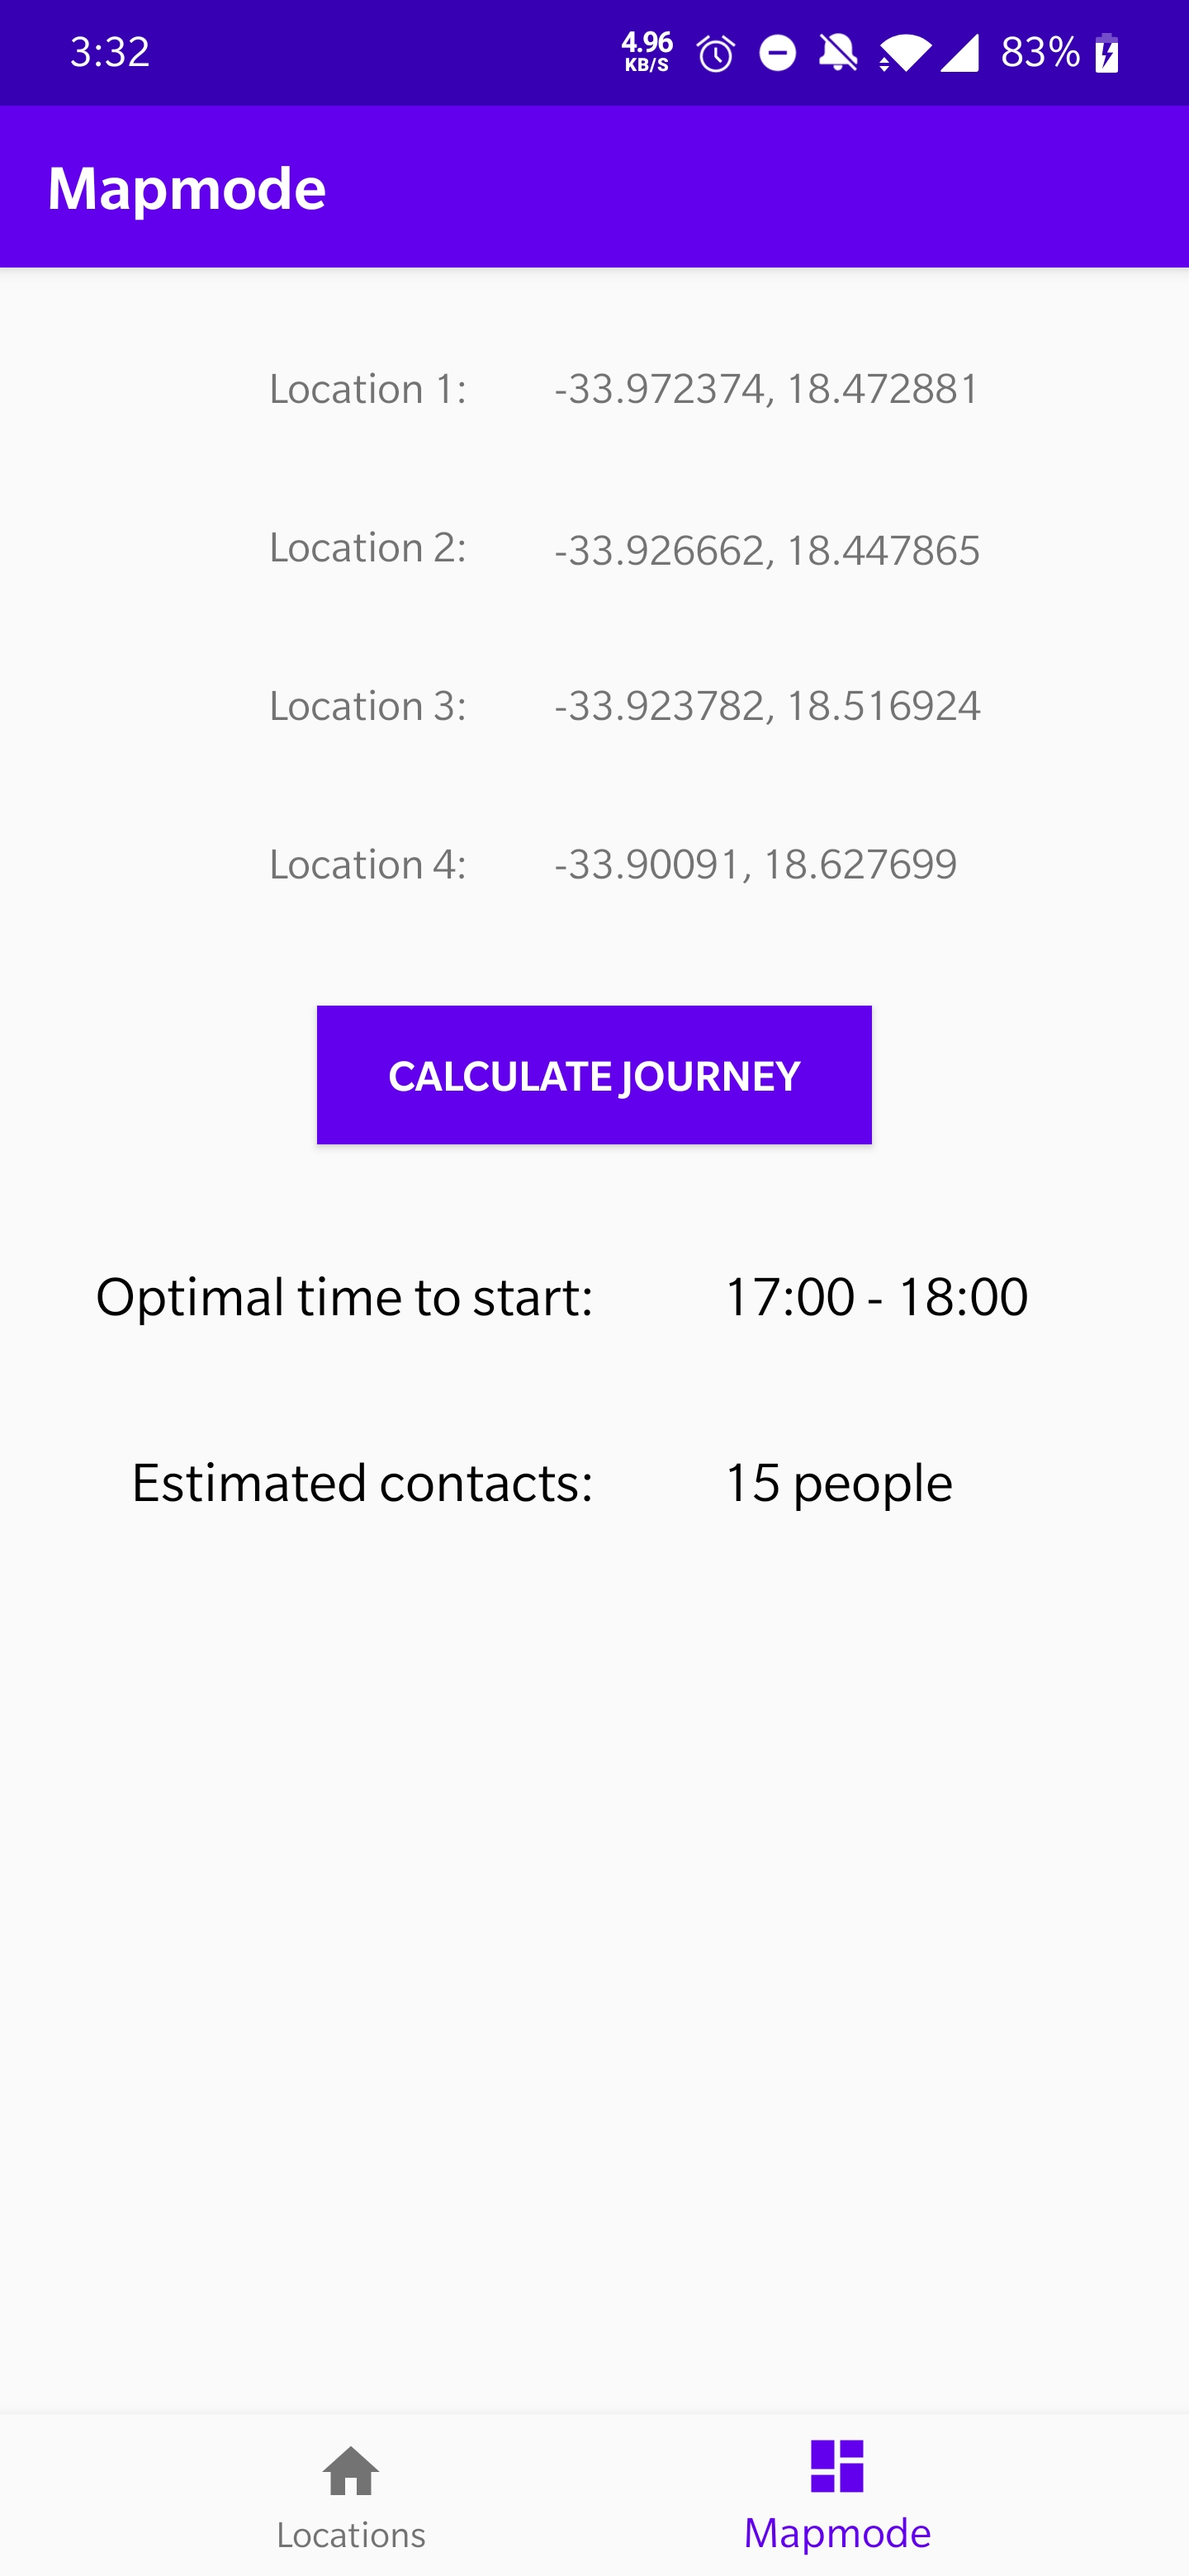
\includegraphics[width=0.25\textwidth]{figures/ResultMapmode.jpg}}
    \caption{Mapmode displaying the optimal start-time and estimated contacts.}
    \label{fig:result_mapmode} 
\end{figure}

A list of user-data was manually inserted into the database for four different locations. The app's Mapmode Fragment was activated to calculate the best time to leave on a journey through each of these locations in order to minimise the number of people whom the user would be near to. The ideal departure time and amount of contact with people was output to the device. The result of the test is displayed in Figure \ref{fig:result_mapmode}.

The control, performed in excel, verifies that the app is able to determine the optimal time to begin the route when minimising person-to-person contact. The raw data and control can be viewed in Appendix \ref{apx:test2}.

\subsubsection{Functional Analysis}

The Location Status and Best Route tests both show that the app can function correctly while providing the user with important population information. This information can be used to make meaningful decisions like when to visit a generally crowded area, how populated a business owner's shops are and when best to go out on your planned trip to minimise the chance of infection. The success of the tests indicate that the app meets its functional requirement of providing a useful service to the user.

\section{Investigative Testing}
\label{sec:Investigative Testing}

TEST-3: \textbf{Location Uncertainty Test}

For this test, a smartphone with the app installed was left in a stationary location for four hours so that it had sufficient time to make location updates. The normal frequency at which the location was uploaded was also artificially increased for the purpose of this test. The scatter of coordinates that were uploaded to the database was recorded and analysed. Because the distribution of the locations is assumed to be gaussian, the uncertainty was calculated using a Type A evaluation. This method uses a combination of the mean and standard deviation to determine the bounds of how accurate the location is. Note that because the smartphone's location is determined by the phone's GPS and network sensor, both the accuracy and uncertainty of location determination will differ from phone to phone.

To determine the uncertainty of the phone's location gathering capabilities, first the coordinate system was zeroed on the mean and each coordinate was converted from degrees into the distance from the mean in meters. This was used to calculate the standard deviation and uncertainty as follows:

\begin{figure}[ht]
    \centering
    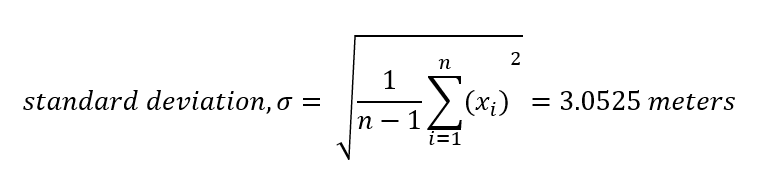
\includegraphics[width=0.6\textwidth]{figures/FormulaSTD.PNG}
    \label{fig:formula_std}
\end{figure}

\begin{figure}[ht]
    \centering
    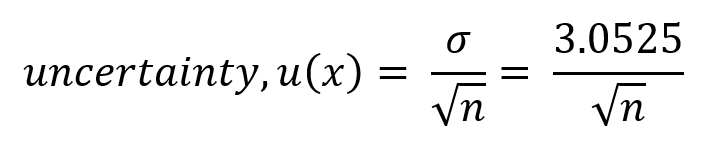
\includegraphics[width=0.4\textwidth]{figures/FormulaUN.PNG}
    \label{fig:formula_std}
\end{figure}

From this result, we can see that the uncertainty of a number of readings is dependent on the number of readings taken. For this test 25 readings were taken which provides an uncertainty of 0.6105 meters. Considering that the PEEPS framework supplies the user with data from locations within 20 meters of their chosen location, an uncertainty of this magnitude is small enough not to have any impact on the functionality of the application. However, if only one reading, n = 1, is used to estimate the user's location, the uncertainty is given to be about 3 meters. While the low uncertainty does not necessarily mean that the device's sensors are accurate, it does mean that once you have a device in a location, the coordinates it uploads will likely be within 3 meters of the mean coordinate. While this variation in location-data is acceptable for this type of crowd-sourced project, it may still be too high for applications where distances in units need to be measured.

TEST-4: \textbf{Upload Regularity Test}

Because the PEEPS framework only functions adequately if the database can receive enough user data, the regularity of the data upload is important for its ability to function reliably. The PEEPS application uses the Android Job Manager to schedule the location upload process, so its timeliness depends on how much priority the Job Manager gives to the process. For this test, the PEEPS application's Job Scheduler set the job's periodic schedule at its normal 15-minute intervals and the phone was left to upload its location over the course of four hours. The timestamps of these uploads were retrieved from the database and their mean was calculated. 

This mean upload interval was determined to be 15.153 minutes. This number is only slightly off the interval set by the Job Scheduler, meaning that the Job Manager is running the service on an interval nearly identical to the one set for it. This result indicates that using a Job Scheduler was the correct method of implementing background services, as it executes reliably. 

TEST-5: \textbf{Smartphone Diagnostic Test}

The app was put through a thorough test lasting 3 minutes using the full functionality of the app. The CPU, memory, network and energy usage were recorded using Android Studio's profiler. Since the profiler does not show averages, they were calculated by sampling the recorded values.

\begin{table}[]
    \centering
    \begin{tabular}{llll}
    \hline
    \textbf{Diagnostic}                                                                & \textbf{Max} & \textbf{Min} & \textbf{Average} \\ \hline
    \begin{tabular}[c]{@{}l@{}}CPU Usage\\ (\% of CPU resources)\end{tabular}          & 17\%         & $\approx$ 0\%        & 4\%              \\ \hline
    Memory Usage                                                                       & 152 MB       & 78 MB        & 107 MB           \\ \hline
    Network Usage                                                                      & 2.4 KB/s     & 0 kb/s       & 0.1 kb/s         \\ \hline
    \begin{tabular}[c]{@{}l@{}}Energy Usage   \\ (profiler energy rating)\end{tabular} & Light        & $\approx$ none       & $\approx$ none           \\ \hline
    \end{tabular}
    \caption{Smartphone diagnostic test results.}
    \label{tab:res_diagnostic}
\end{table}

The application is built to be lightweight in terms of its processing requirements and this is mirrored in the results of this test. While the CPU usage does spike to 17\% at its maximum, the average CPU usage of 4\% means that the application will not put a large load on the phone's capabilities. Even if the average CPU usage was closer to the maximum, since the app is running in the foreground, one would assume it would make use of most of the phone's resources, but this is not the case. The memory usage is small enough to take up a negligible amount of the phone's total RAM.

\subsubsection{Investigative Analysis}

The investigative testing implies that the PEEPS framework meets the goal of it being lightweight, scalable and sufficiently accurate. In particular, the uncertainty of the location gathering mechanism, determined by TEST-3, is a promising result for developers wishing to work with closer proximities than PEEPS's 20-meter radius. A 0.6105-meter uncertainty, determined over the course of 25 readings, means that location uploading services could even target specific locations and determine if a person is in that area. This can be incredibly useful for businesses to determine whether an employee is at their station or for IoT devices to determine events, like whether a person has left their bed. 

The strict interval of the location upload process is also promising for developers wanting a service that requires strict regularity. While the PEEPS service does not need minute precision, apps that do will find that the JobService functionality of Android applications is reliable enough for this purpose, while also having runtime customisation from network status to battery power. 

While Android Studio's profiler is limited in its analysis, the usage data it provided indicates that this app is lightweight in terms of both network and smartphone resource usage. This is ideal, as the objective is to have an app that can be installed and used on any compatible device. While the test smartphone can be considered high-end, the diagnostic results indicate that the phone's processing ability is not a major concern.

\section{Verification of Specifications}

\subsubsection{Mobile Application Specifications}

\begin{SA}
    \item General Specifications
    \begin{SA}
        \item App must be able to run on any version of Android between 6 and 10. \textbf{Fulfilled.}
    \end{SA}
    \item Graphical User Interface 
    \begin{SA}
        \item Must follow a consistent colour pallet with a primary and secondary colour selection. \textbf{Fulfilled.}
        \item All user interactions with the app must be clearly interpretable from the GUI. \textbf{Fulfilled.}
        \item Buttons must be placed below text inputs in each activity or on the toolbar. \textbf{Fulfilled.}
    \end{SA}
    \item Location Services
    \begin{SA}
        \item Location must be uploaded to server at regular intervals. \textbf{Fulfilled.}
        \item Location upload interval must be shorter than 20 minutes. \textbf{Fulfilled.}
        \item Location data is uploaded when app is minimised. \textbf{Fulfilled.}
        \item Location data is uploaded when app is closed. \textbf{Fulfilled.}
        \item Location data upload starts on smartphone boot if user has logged in previously. \textbf{Fulfilled.}
    \end{SA}
    \item User interaction
    \begin{SA}
        \item User will be able to save ‘favourite' locations by entering their coordinates or address. \textbf{Partially fulfilled. No address searching.}
        \item Saved locations will be stored locally using an SQL database. \textbf{Fulfilled.}
        \item Saved locations will display current population density status on the app's main page. \textbf{Fulfilled.}
        \item When selected, saved locations will display a graph showing the level of activity at that location for that day, as well as the predicted activity for the rest of the day. \textbf{Fulfilled.}
    \end{SA}
    \item Data security
    \begin{SA}
        \item User will need to login with correct username and password to access application. \textbf{Fulfilled.}
        \item No population density data displayed on the app will contain information about the user who uploaded it. \textbf{Fulfilled.}
    \end{SA}
\end{SA}

\subsubsection{Database Specifications}

\begin{SA}
    \item General Specifications
    \begin{SA}
        \item Database will be secured with appropriate password. \textbf{Fulfilled.}
    \end{SA}
    \item Tables
    \begin{SA}
        \item Database will contain a table storing users' login data. \textbf{Fulfilled.}
        \item Database will contain a table storing users' geographical data. \textbf{Fulfilled.}
        \item Location table will require timestamps for each location stored as well as the username of the user who uploaded it. \textbf{Fulfilled, although username isn't checked by database.}
    \end{SA}
\end{SA}

\subsubsection{Web Interface Specifications}

\begin{SA}
    \item General Specifications
    \begin{SA}
        \item Server is accessible from devices outside its home network. \textbf{Not fulfilled. Server needs to be on same home network as device.}
    \end{SA}
    \item Data Communication
    \begin{SA}
        \item User and geographical data sent to the server must be checked for database compatibility. \textbf{Partially fulfilled.}
        \item Data sent to the server, if valid, will be stored on the connected database. \textbf{Fulfilled.}
        \item All location data processing will be done by the server, and only results will be forwarded to the application. \textbf{Partially fulfilled, much data proccessing still done by the app.}
    \end{SA}
    \item Security
    \begin{SA}
        \item Data retrieved by the app from other users via the server must be anonymous. \textbf{Fulfilled.}
    \end{SA}
\end{SA}

\section{Discussion}

Since the purpose of this project was to investigate the PEEPS's ability to correctly predict population density, the functional testing centred around trying to investigate whether this was accomplished successfully. The results of these functional tests indicate that this project goal was accomplished. Both the Saved-Location and Mapmode views provided the user with visually appealing user interfaces which the user could use to get actionable insight into the population density of chosen locations. The Saved-Location view was particularly successful as it allowed the user fine control over the locations they wished to analyse while also providing the predicted population for most of the day, based on past population densities. While the Mapmode view worked as intended, it acted as more of a test of the app's capabilities when dealing with large amounts of location data and processing time. The results from TEST-2 indicate that this fragment was able to correctly calculate the optimal time to begin a journey and the number of predicted contacts. Since the functionality of this view is proven, it could now be redesigned with user interaction in mind. 

The investigative testing revealed useful information about both app development and Android's location services. The Fused Location Provider used by the app to find its current location was found to have a standard deviation of 3.0525 meters which is a value that is vital to know when designing location-determining apps. Any Android application using this fused-location service should be aware that the coordinate value determined will vary about two standard deviations\footnote{For 95.4\% of values.} from the mean. The standard deviation value is very similar to the average uncertainty calculated by the Warnell School of Forestry and Natural Resources using the iPhone 6, which found that most values varied between 3 meters of the mean error amount \cite{Merry2019}. The investigative testing also determined the reliability of the Android's background Job Service Schedular and the lightweight execution of the PEEPS app. The latter is promising for developers wanting to use location tools in the background of a resource intensive app, as the location services used in this project were not CPU, network, memory, or battery intensive.  